% !TEX root = ./Vorlesungsmitschrift DIFF 2.tex  
\lecture{Do 04.06. 10:15}{}
Letztes Mal: Untermannigfaltigkeiten \emph{lokal} als Nullstellengebilde (Definition), als Graph und als diffeomorph zu Teilmengen des des \( \reals^d\times\zeroset \).

Eine weitere äquivalente lokale Beschreibung mit Hilfe einer Parametisierung:
\begin{definition}\index{Immersion}
  Eine Abbildung \( \varphi\maps V\to \reals^n \), \( V\subset \reals^d \) offen, \( d\leq n \), heißt \emph{Immersion}, falls sie stetig differenzierbar ist und der Rang von \( D\varphi(t) \) für alle \( t\in V \) maximal, also gleich \( d \) ist. Man nennt \( \varphi(V) \) die \emph{Spur} von \( \varphi \). Ist \( \varphi\maps V\to \varphi(V) \) ein Homöomorphismus (also stetig, bijektiv, mit stetigem Inversen), so heißt \( \varphi \) \emph{Einbettung}. 
\end{definition}
\begin{beispiele*}
  \begin{enumerate}[label=\rechtsklammer{\roman*}]
    \item \label{immersion_beispiel:schlenkel_kurve} \( V=\reals \), \( \phi(t)=(t^2-1,t(t^2-1)) \). 
    \begin{figure}[H]
      \centering
      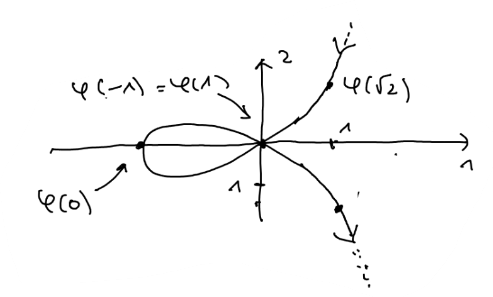
\includegraphics[width=0.5\linewidth]{immersion_schlenkel_kurve_keine_einbettung}
      \label{fig:immersion_schlenkel_kurve_keine_einbettung}
    \end{figure}
    \begin{align*}
      \varphi(1)&=(0,0)=\phi(-1)\qquad \text{also keine Einbettung}\\
      \varphi(0)&=(-1,0)\\
      \varphi(\sqrt{2})&=(1,\sqrt{2})\\
      \varphi(-t)&=(\phi_1(t),-\phi_2(t))\\[1ex]
      \varphi'(t)&=(2t,\braceannotate{\neq 0 \text{ für }t\neq \frac{1}{\sqrt{3}}}{3t^2-1})\neq 0\implies \text{maximaler Rang}.
    \end{align*}
    Eine Immersion \( \varphi\maps I\subset \reals\to \reals^n \) heißt auch \emph{reguläre (parametisierte) Kurve}.
    
    \begin{bemerkung*}
      \( 1 \)-dimensional \tto \( I \) kann auch nicht offen gewählt werden, wenn man nur an Differenzierbarkeit interessiert ist. Hier \emph{nicht}.
    \end{bemerkung*}
    \item \( V=\Set{t\in \reals^2|\euclidiannorm{t}<1} \), \( \varphi(t_1,t_2)=\transpose-{(t_1,t_2,\sqrt{1-t_1^2-t_2^2})} \),  
    \begin{equation*}
      D\varphi(t_1,t_2)=\begin{pNiceMatrix} \Block{1-2}{\mathds{1}_{2\times 2}} \\ \frac{-t_1}{\sqrt{\cdots}} & \frac{-t_2}{\sqrt{\cdots}}  \end{pNiceMatrix}\qquad \rang;=2\quad \forall t\in V.
    \end{equation*}
    \begin{figure}[H]
      \centering
      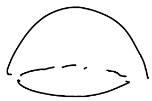
\includegraphics[width=0.5\linewidth]{immersion_halbkugel}
      \caption*{Spur von \( \varphi \).}
      \label{fig:immersion_halbkugel}
    \end{figure}
    \item \label{immersion_beispiel:kugel}\( V=\ointerval{0}{\pi}\times \ointerval{0}{2\pi} \),
    \begin{equation*}
      \varphi(\beta,\alpha)=(\Cos{\alpha}\Sin{\beta},\Sin{\alpha}\Sin{\beta},\Cos{\beta}).
    \end{equation*}
    \begin{figure}[H]
      \centering
      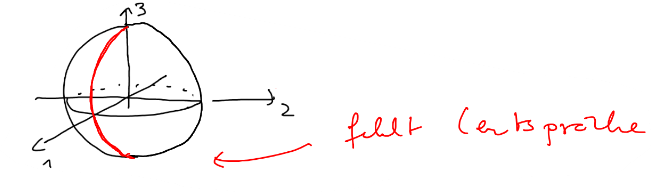
\includegraphics[width=0.5\linewidth]{immersion_kugel}
      \caption*{Spur von \( \varphi \)}
      \label{fig:immersion_kugel}
    \end{figure}
    \( V=\reals^2 \), \( \varphi \) wie oben: \( \varphi \) schneidet sich \( \infty \) oft, da \( \varphi(\beta+2\pi \wholes,\alpha+2\pi\wholes)=\phi(\beta,\alpha ) \) gilt. \( \varphi(\reals^2)=\sphere{2} \).
  \end{enumerate}
\end{beispiele*}
\begin{satz}\label{immersion_ist_lokal_einbettung_und_mannigfaltigkeit}
  Sei \( \varphi\maps V\to \reals^n \), \( V\subset \reals^d \), eine Immersion. Dann gibt es zu jede, \( t_0\in V \) eine offene Umgebung \( V_0\subset V \) \sd \( \evaluateat{\varphi}{V_0} \) eine Einbettung des \( \reals^n \) ist und \( \varphi(V_0) \) eine \( d \)-dimensionale Untermannigfaltigkeit des \( \reals^n \).
\end{satz}
\begin{proof}
  Nach eventueller Umnummerierung der Komponenten von \( \varphi \). Sei
  \begin{equation*}
    \begin{pNiceMatrix}
      \partial_1 \varphi_1 & \Cdots & \partial_d \varphi_1(t_0) \\
      \Vdots &  & \Vdots \\
      \partial_1 \varphi_d(t_0) & \Cdots & \partial_d \varphi_d(t_0)
    \end{pNiceMatrix}
  \end{equation*}
  invertierbar.

  Dann gibt es nach dem Satz über die Umkehrfunktion \thref{satz_von_der_umkehrabbildung} offene Umgebungen \( V_0 \subset \reals^d\) von \( t_0 \) und \( W\subset \reals^d \) von \( \begin{pNiceMatrix} \varphi_1(t_0) \\ \Vdots \\ \varphi_d(t_0) \end{pNiceMatrix} \) \sd
  \begin{equation*}
    \tilde{\varphi}=\begin{pNiceMatrix} \varphi_1 \\ \Vdots \\ \varphi_d \end{pNiceMatrix}\maps V_0\to W
  \end{equation*}
  Diffeomorphismus ist (also stetig differenzierbar mit stetig differenzierbarem Inversen). Wir zeigen, dass \( \varphi(V_0) \) diffeomorph ist zu \( V_0\times \zeroset \). Dann folgt aus \thref{mannigfaltigkeit_sieht_lokal_aus_wie_r_n}, dass \( \varphi(V_0) \) \( d \)-dimensionale Untermannigfaltigkeit des \( \reals^n \) ist.
  \begin{subproof}
    Setze dazu \( G\maps V_0\times \reals^{n-d}\to \reals^d\times \reals^{n-d} \).
    \begin{equation*}
      G(\braceannotate{t}{t',t''})\definedas \begin{pNiceMatrix} \varphi_1(t') \\ \Vdots \\ \varphi_d \\ \varphi_{d+1}(t')+t_{d+1}\\ \Vdots \\ \varphi_{d+1}(t')+t_n \end{pNiceMatrix}=\begin{pNiceMatrix}\tilde{\varphi}(t') \\ \tilde{\tilde{\varphi}}(t') +t'' \end{pNiceMatrix}\qquad \tilde{\tilde{\varphi}}=\begin{pNiceMatrix} \varphi_{d+1} \\ \Vdots \\ \varphi_n \end{pNiceMatrix}.
    \end{equation*}
    Dann ist \( G(V_0\times\reals^{n-d})=W\times\reals^{n-d} \), denn
    \begin{proofdescription}
      \item[\sethin] ist klar, da \( \tilde{\varphi}\maps V_0\to W \) Diffeomorphismus ist.
      \item[\setrueck] Sei \( (y,y'')\in W\times\reals^{n-d} \). Setze \( t'=\inverse{\tilde{\varphi}}(y') \) (\( \tilde{\varphi}\maps V_0\to W \) Diffeomorphismus), \( t''=y''-\tilde{\tilde{\varphi}}(t') \). Dann gilt \( G(t',t'')=\begin{pNiceMatrix} y' \\ y'' \end{pNiceMatrix} \).
    \end{proofdescription}
    Man sieht:  \( G\maps V_0\times\reals^{n-d}\to W\times\reals^{n-d} \) ist bijektiv. Man sieht auch sofort: \( G \) ist Diffeomorphismus, da \( \tilde{\varphi} \) Diffeomorphismus ist und \( \tilde{\tilde{\varphi}} \) stetig differenzierbar und somit auch die Umkehrfunktion
    \begin{equation*}
      F(y',y'')=\begin{pNiceMatrix} \inverse{\tilde{\varphi}}(y') \\ y''-\tilde{\tilde{\varphi}}(\inverse{\tilde{\varphi}}(y)) \end{pNiceMatrix}
    \end{equation*}
    stetig differenzierbar ist. Wegen \( G(V_0\times \zeroset) =\varphi(V_0)\) \( d \)-dimensionale Untermannigfaltigkeiten.
  \end{subproof}
  Es folgt auch, dass \( \evaluateat{\varphi}{V_0} \) Einbettung ist:
  
  Denn \(\evaluateat{\tilde{\varphi}}{V_0}  \)
   ist Diffeomorphismus (auf \( W \)) und somit ist
    \( \evaluateat{\varphi}{V_0} \) 
    injektiv. Wegen 
    \( \varphi(t)=G(t,0) \) 
    ist die Umkehrfunktion
     \( \inverse{\varphi}\maps \varphi(V_0)\to \reals^n \) 
     stetig.
\end{proof}
\begin{beispiel*}[Beispiel~\ref{immersion_beispiel:schlenkel_kurve}]
  Wegen \( \phi(1)=\varphi(-1) \) ist \( \varphi \) keine Einbettung. Es ist auch kein Untermannigfaltigkeit, was man hier leichter als in Aufgabe 2 auf Blatt 7 sieht: Es gibt \( 2 \) linear unabhängige Tangentialvektoren an \( (0,0) \), \zb \( \varphi'(1)=(2,2) \), \( \varphi'(-1)=(-2,2) \). \timestamp{9:15}
  
  Wählt man aber etwa \( I_0=\ointerval{-\frac{1}{2}}{\infty} \), so erhält man
  \begin{figure}[H]
    \centering
    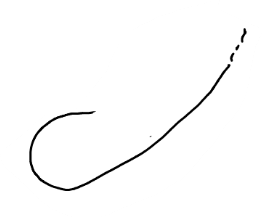
\includegraphics[width=0.5\linewidth]{immersion_schlenkel_kurve_keine_einbettung_ohne_doppelpunkt}
    \label{fig:immersion_schlenkel_kurve_keine_einbettung_ohne_doppelpunkt}
  \end{figure}
  ohne Doppelpunkt.
\end{beispiel*}
Tatsächlich gilt:
\begin{satz}\label{mannigfaltigkeiten_sind_parametisierbar}
  Eine Teilmenge \( M\subset \reals^n \) ist genau dann eine \( d \)-dimensionale Untermannigfaltigkeit des \( \reals^n \), wenn es zu jedem Punkt \( a\in M \) eine offene Umgebung \( U\subset \reals^n \) von \( a \) gibt und eine offene Teilmenge \( V\subset \reals^d \) und eine Einbettung \( \varphi\maps V\to \reals^n \) mit \( \varphi(V)=M\cap U \).
\end{satz}
\begin{proof}
  \begin{proofdescription}
    \item[\rueck] Sei also \( a\in M \) und \( U \), \( \varphi\maps V\to \reals^n \) wie oben, \( a>\varphi(t_0) \). Dann gibt es (\thref{immersion_ist_lokal_einbettung_und_mannigfaltigkeit}) eine offene Umgebung \( V_0 \) von \( t_0 \) \sd \( \varphi(V_0) \) eine \( d \)-dimensionale Untermannigfaltigkeit ist. Es ist \( \varphi(V_0)\subset M\cap U \) offen, (nach dem Satz von der offenen Abbildung) \timplies Es gibt eine offene Umgebung \( U_0 \) von \( \varphi(t_0)=a \) \sd \( \varphi(V_0)=M\cap U_0 \) \timplies \( M\cap U_0 \) ist \( d \)-dimensionale Untermannigfaltigkeit. Da man dies für jeden Punkt \( a\in M \) machen kann, folgt: \( M \) ist \( d \)-dimensionale Untermannigfaltigkeit.
    \item[\hin] Wir schreiben \( M \) lokal als Graphen: \( a\in U=U_1\times U_2\subset \reals^d\times\reals^{n-d} \),   
    \begin{equation*}
      M\cap U=\Set{(x',g(x'))|x'\in U_1}.
    \end{equation*}
    Setze \( V\definedas U_1 \) und \( \varphi\maps V\to \reals^n \), \( \varphi(t)=\transpose-{(t,g(t))} \). Dann ist \( \varphi \) eine Immersion (denn \( D\varphi(t)=\begin{pNiceMatrix} \mathds{1}_{d\times d} \\ Dg(t) \end{pNiceMatrix} \) hat maximalen Rang) mit \( \varphi(V)=M\cap U \) (da \( g(V)=U_2 \)). \( \varphi \) ist injektiv und die Umkehrfunktion
      \begin{equation*}
        \inverse{\varphi}\maps \equalto{U_1\times U_2}{\varphi(V)}\to \reals^d,\quad (y',y'')\mapsto y'
      \end{equation*}
      ist stetig.
  \end{proofdescription}
  
\end{proof}
\begin{bemerkungen*}
  \item Man nennt \( \varphi \) wie oben eine \emph{lokale Parametrisierung} von \( M \) bei \( a \). \( V \) heißt \emph{Parameterbereich} und \( M\cap U \) \emph{Koordinatenumgebung von \( a \)}.
  \item Globale Parametisierungen \( \varphi\maps V\to\reals^n \) mit \( \varphi\maps V\to M \). Homöomorphismus existieren \ia nicht.
  \begin{beispiel*}
    \( M=\sphere{n-1}\subset \reals^n \). Es kann keine stetige Abbildung \( \inv{\varphi}\maps \sphere{n-1}\to V \) gebe, da \( \inv{\varphi}(\sphere{n-1}) \) kompakt wäre, aber \( V \) ist offen.
    
    Im Beispiel~\ref{immersion_beispiel:kugel} oben, erreicht man daher nicht die ganze \( \sphere{n} \). \( V=\ointerval{0}{\pi}\times \ointerval{0}{2\pi} \),
    \begin{equation*}
      \varphi(\beta,\alpha)=(\Cos{\alpha}\Sin{\beta},\Sin{\alpha}\Sin{\beta},\Cos{\beta}).
    \end{equation*}
    \begin{figure}[H]
      \centering
      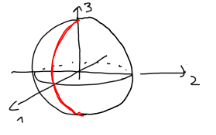
\includegraphics[width=0.5\linewidth]{immersion_kugel_einfach}
      \caption*{Spur von \( \varphi \)}
      \label{fig:immersion_kugel_einfach}
    \end{figure}
    oder (\( V=\reals^2 \)) es liegt kein Homöomorphismus vor.

    Für \( a\in \Set{(\Sin{\beta},0,\Cos{\beta})|\beta\in \ointerval{0}{\pi}} \) wählt man als lokale Parametisierung einfach \( V=\ointerval{0}{\pi}\times \ointerval{-\pi}{\pi} \) (dann fehlt ein anderer Halbkreis).

    Oder man wählt \( D\ni (y,z)\mapsto (\sqrt{1-y^2-z^2},y,z) \) mit
    \begin{equation*}
      D=\Set{(y,z)\in \reals^2|\euclidiannorm{(y,z)}<1}.
    \end{equation*}
  \end{beispiel*}
\end{bemerkungen*}
\begin{satz}[Parameterwechsel]\label{parameterwechsel}\approxtimestamp{29}\index{Parameterwechsel}
  Sei \( M\subset \reals^n \) eine \( d \)-dimensionale Untermannigfaltigkeit. Seien \( \varphi\maps V\to M\cap U \) und \( \psi\maps \tilde{V}\to M\cap \tilde{U} \) zwei lokale Parametisierungen mit \( M\cap U\cap \tilde{U}\neq \emptyset \). Dann ist der \emph{Parameterwechsel}   
  \begin{equation*}
    \inverse{\psi}\circ \varphi\maps \inv{\varphi}(M\cap U\cap \tilde{U})\to \inverse{\psi}(M\cap U\cap \tilde{U})
  \end{equation*}
  ein Diffeomorphismus.
\end{satz}
\begin{bemerkungen*}
  \( \inverse{\varphi}(M\cap U\cap \tilde{U}) \) und \( \inverse{\psi}(M\cap U\cap \tilde{U}) \) sind offen.
\end{bemerkungen*}
\begin{figure}[H]
  \centering
  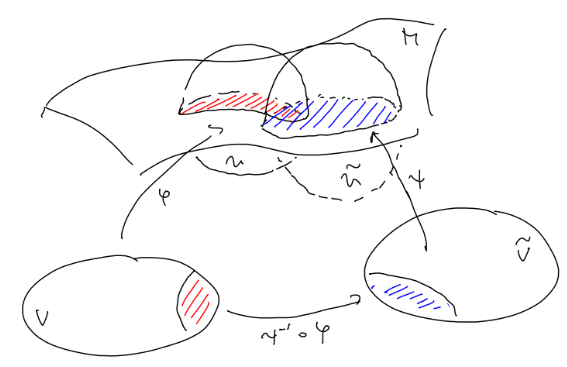
\includegraphics[width=\linewidth]{reparametisierung_intuition}
  \label{fig:reparametisierung_intuition}
\end{figure}
\begin{proof}
  Da \( \varphi \) und \( \psi \) stetig sind, und \( M\cap U \) und \( M\cap \tilde{U} \) offen, sind \( \inverse{\varphi}(M\cap U\cap \tilde{U}) \) und \( \inverse{\psi}(M\cap U\cap \tilde{U}) \) offen.
  
  \( \inverse{\psi}\circ \varphi \) ist als Komposition von Homöomorphismen Homöomorphismus.

  Sei \( a\in M\cap U\cap \tilde{U} \), \( t_0\definedas \inverse{\varphi}(a) \), \( \tilde{t}_0\definedas \inverse{\psi}(a) \). \( M \) ist lokal diffeomorph zu einem Ebenenstück \timplies \texists  offene Umgebung \( U(a) \) von \( a \) und eine offene Teilmenge \( W\subset \reals^n \) \sd und ein Diffeomorphismus \( 
    F\maps U(a)\to W \) \sd
    \begin{equation*}
      F(M\cap U(a))=\Set{y\in W|y_{d+1}=\dotsb=y_n=0}.
    \end{equation*}
  Ohne Einschränkung nehmen wir an, dass 
  \begin{equation*}
    U(a)\subseteq U\cap \tilde{U}
  \end{equation*}
  gilt. Dann gilt auf \( \inverse{\varphi}(M\cap U\cap \tilde{U}) \)
  \begin{equation*}
    F\circ \varphi=(h_1,\dotsc,h_d,0,\dotsc,0)
  \end{equation*}
  und auf \( \inverse{\psi}(M\cap U\cap \tilde{U}) \)
  \begin{equation*}
    F\circ \psi=(f_1,\dotsc,f_d,0,\dotsc,0)
  \end{equation*}
  und \( D(F\circ \varphi) \) und \( D(F\circ \psi) \) haben Rang \( d \), da \( DF \) Rang \( n \) hat und \( D\varphi \) und \( D\psi \) Rang \( d \).
  \begin{equation*}
    \implies (h,0)\maps \inverse{\varphi}(M\cap U\cap \tilde{U})\to \Set{y\in W|y_j=0\quad j\geq d+1}
  \end{equation*}
  und
  \begin{equation*}
    (f,0)\maps \inverse{\varphi}(M\cap U\cap \tilde{U})\to \Set{y\in W|y_j=0\qquad j\geq d+1}
  \end{equation*}
  sind Diffeomorphismen. Auf \( \inverse{\varphi}(M\cap U\cap \tilde{U}) \) gilt
  \begin{equation*}
    \inverse{\psi}\circ \varphi=\inverse{(F\circ \psi)}\circ (F\circ \varphi)=\inverse{(f,0)}\circ (h,0),
  \end{equation*}
  also ist \( \inverse{\psi}\circ \varphi \) Diffeomorphismus.
  \begin{figure}[H]
    \centering
    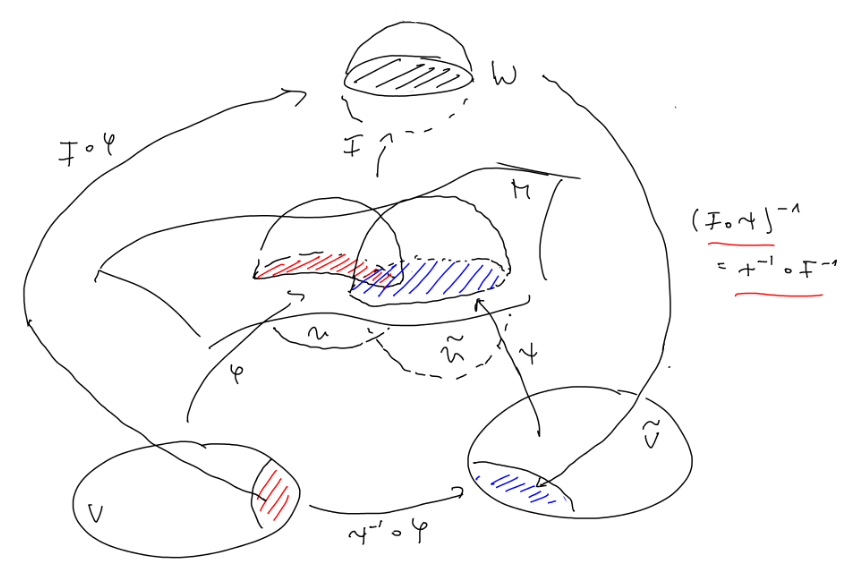
\includegraphics[width=\linewidth]{reparametisierung_beweis}
    \label{fig:reparametisierung_beweis}
  \end{figure}
\end{proof}
